\section{Results}
\subsection{Research question 1}
For research question 1 the results are 2-dimensional plotted using a line diagram.

\subsubsection{Utility}
\begin{figure}[!htb]
  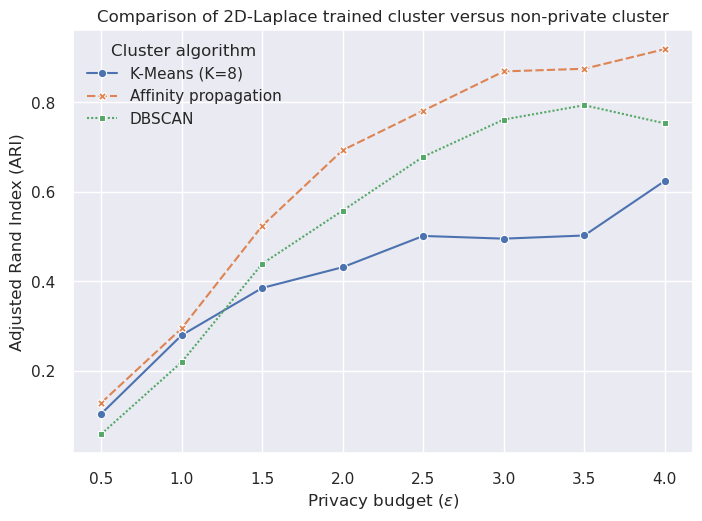
\includegraphics[width=0.7\linewidth]{Results/ARI-epsilons.png}
  \caption{ARI evaluation for cluster algorithms 2D-Laplace for a dataset with shape (50, 2)}
\end{figure}
\begin{figure}[!htb]
  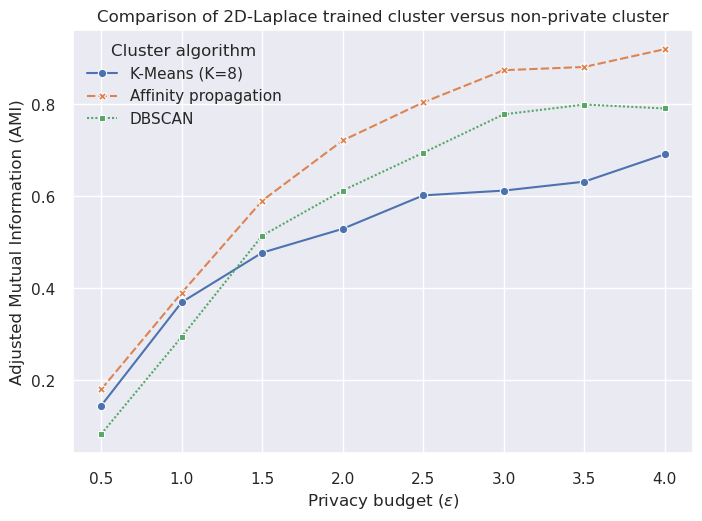
\includegraphics[width=0.7\linewidth]{Results/AMI-epsilons.png}
  \caption{AMI evaluation for cluster algorithms trained with 2D-Laplace for a dataset with shape (50, 2)}
\end{figure}
\newpage
\subsubsection{Privacy}
\begin{table}[h]
  \caption{Geo-indistinguishability as an error metric}
  \begin{tabular}{lrrr}
     & epsilon & average p\_e & distance \\
     & 0.05    & 0.447944     & 3.854884 \\
     & 0.1     & 0.397897     & 3.761739 \\
     & 0.2     & 0.309593     & 2.899825 \\
     & 0.3     & 0.240543     & 3.234295 \\
     & 0.4     & 0.189171     & 2.508862 \\
     & 0.5     & 0.151567     & 2.461655 \\
     & 1       & 0.067893     & 1.282425 \\
     & 1.5     & 0.043456     & 1.178248 \\
     & 2       & 0.032263     & 0.900766 \\
     & 2       & 0.025261     & 0.591023 \\
     & 3       & 0.020199     & 0.645654 \\
  \end{tabular}
\end{table}
\subsection{Research question 2}
\subsection{Research question 3}